\subsection{Časovače a počítadlá}
\noindent

Ako názov napovedá, časovače sú určené na meranie času. Často ich nazývame aj počítadlá
pretože vo svojom základnom princípe časovače len počítajú počet dokončených periód zdrojových hodín.
Každý časovač má svoj vlastný register, kde je uložená jeho aktuálna hodnota a taktiež každý potrebuje zdroj hodín. V mikrokontroléroch často existuje niekoľko možných zdrojov
hodín a ich výber je možné určiť pomocou prepínača. Niektoré mikrokontroléry umožňujú aj použitie
externých hodín \cite{IntroductionMicrocontrollerTimers}. \par
Fungovanie časovača si najlepšie opíšeme na konkrétnom príklade.
Uvažujme časovač s 16-bitovým registrom a zdrojom hodín s frekvenciou 16 megahertzov. Po každom uplynutí cyklu v hodinách, časovač
zvýši hodnotu uloženú v registri o 1. Keďže časovač má k dispozícii 16-bitový register, maximálny počet možných hodnôt v registri je $2^{16}$ (65536).
Po dosiahnutí maximálnej hodnoty register pretečie a časovač začne počítať znova od 0. Ten proces sa opakuje stále dookola a zmena hodnoty v
registri je zobrazená na obrázku č.\ref{figure:timer1}.

\begin{figure}[!h]
    \centering
    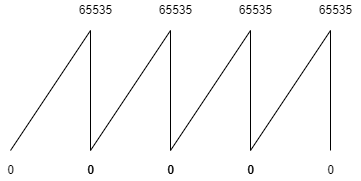
\includegraphics{img/timer.png}
    \caption{Zmena hodnota v 16 bitovom registri časovača.}
    \label{figure:timer1}
\end{figure}